% !TEX root = Apostila GP.tex

\capitulo{Riscos}

\secao{Objetivos e características}

O gerenciamento dos riscos do projeto inclui os processos necessários para aumentar a probabilidade e impacto de eventos positivos e diminuir a probabilidade de eventos negativos no projeto.

Os processos que fazem parte do gerenciamento dos riscos, representados na Figura \ref{fig:proc:ger:riscos}, podem ser resumidos em:

\begin{description}
	
	\item[Planejar o gerenciamento dos riscos:] definir como conduzir as atividades de gerenciamento de riscos para o projeto.

	\item[Identificar os riscos:] determinar quais riscos podem afetar o projeto e documentar suas características.

	\item[Realizar a análise qualitativa dos riscos:]  avaliar a exposição ao risco para priorizar os riscos que serão objeto de análise ou ação adicional.

	\item[Realizar a análise quantitativa dos riscos:] efetuar a análise numérica do efeito dos riscos identificados nos objetivos gerais do projeto.

	\item[Planejar as respostas aos riscos:] desenvolver opções e ações para aumentar as oportunidades e reduzir as ameaças aos objetivos do projeto.

	\item[Controlar os riscos:] monitorar e controlar os riscos durante o ciclo de vida do projeto.	

\end{description}

\begin{figure}[!h]
	\centering
	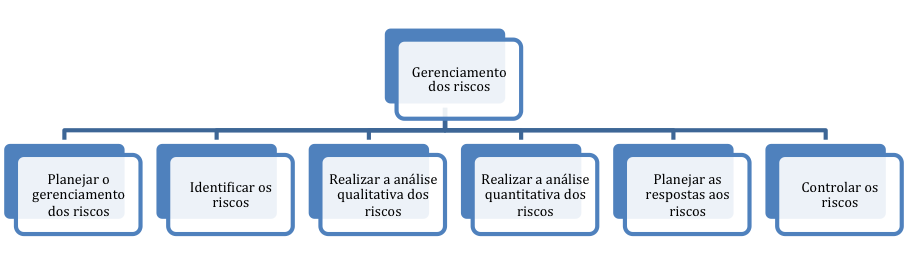
\includegraphics[scale=0.75]{Figuras/gerenciamento_riscos.png}
	\caption{Processos do Gerenciamento dos riscos}
	\label{fig:proc:ger:riscos}
\end{figure}

\secao{Planejar gerenciamento dos riscos}

O plano de gerenciamento dos riscos é o processo de como conduzir as atividades de gerenciamento dos riscos para um projeto.

O processo de planejar o gerenciamento dos riscos está representado na Figura \ref{fig:riscos:plan:efts} e será descrito a seguir.

\begin{figure}[!h]
	\centering
	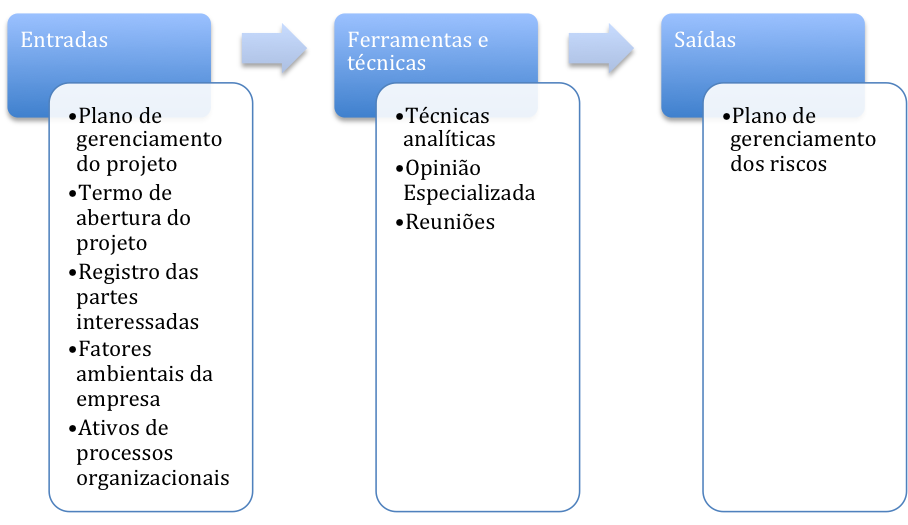
\includegraphics[scale=0.5]{Figuras/riscos_efts_planejar.png}
	\caption{Planejar o gerenciamento dos riscos: entradas, ferramentas, técnicas e saídas}
	\label{fig:riscos:plan:efts}
\end{figure}

\section{Entradas}

\begin{description}
	
	\item[Plano de gerenciamento do projeto:] todos os planos de gerenciamento subsidiários e linhas de base devem ser levados em consideração a fim de fazer com que o plano de gerenciamento de riscos esteja consistente com eles.
	
	\item[Termo de abertura do projeto:] contém os riscos em alto nível, descrições do projeto, requisitos de alto nível, etc.
	
	\item[Registro das partes interessadas:] oferece uma visão geral dos papéis das partes interessadas.
	
	\item[Fatores ambientais da empresa:] inclui atitudes, limites e tolerâncias aos riscos que caracterizam a resistência ao risco da organização.
	
	\item[Ativos de processos organizacionais:] categorias de riscos, definições de conceitos e termos, formatos de declaração de riscos, modelos, papéis e responsabilidades, nível de autoridade para tomada de decisões, lições aprendidas, etc.

\end{description}

\section{Ferramentas e técnicas}

\begin{description}

	\item[Técnicas analíticas:] utilizadas para entender e definir a visão geral do contexto do gerenciamento de riscos do projeto.
	
	\item[Opinião Especializada:] para garantir o estabelecimento compreensivo do plano de gerenciamento de riscos.
	
	\item[Reuniões:] para desenvolver o plano de gerenciamento de riscos.
	
\end{description}

\section{Saídas}

\begin{description}
	
	\item[Plano de gerenciamento dos riscos:] descreve como as atividade de gerenciamento de riscos serão estruturadas e realizadas.
	
\end{description}

\secao{Identificar os riscos}

Processo de determinar quais riscos podem afetar o projeto e documentar suas características.

O processo de identificar os riscos está representado na Figura \ref{fig:riscos:ident:efts} e será descrito a seguir.

\begin{figure}[!h]
	\centering
	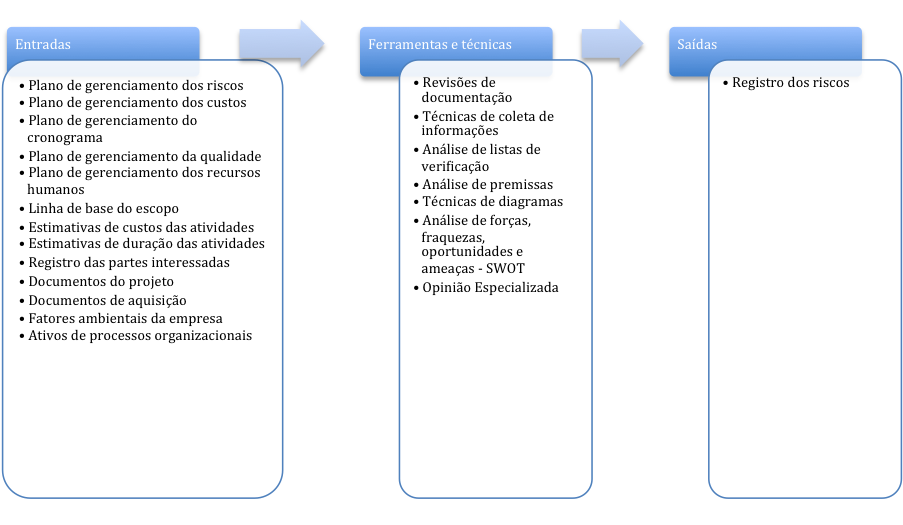
\includegraphics[scale=0.5]{Figuras/riscos_efts_identificar.png}
	\caption{Identificar os riscos: entradas, ferramentas, técnicas e saídas}
	\label{fig:riscos:ident:efts}
\end{figure}

\section{Entradas}

\begin{description}
	
	\item[Plano de gerenciamento dos riscos:] oferece elementos chave, tais como papéis e responsabilidades atribuídas, provisão no orçamento e cronograma para atividades de gerenciamento de riscos e categorias de riscos.
	
	\item[Plano de gerenciamento dos custos:] contém processos e controles que podem ser usados no auxílio da identificação de riscos.
	
	\item[Plano de gerenciamento do cronograma:] contém objetivos de cronograma que podem ser impactados pelos riscos.
	
	\item[Plano de gerenciamento da qualidade:] contém uma linha de base de medidas e métricas de qualidade para uso na identificação dos riscos.
	
	\item[Plano de gerenciamento dos recursos humanos:] contém papéis e responsabilidades, organogramas e planejamento de gerência de pessoal que são entradas chave para o processo de identificação dos riscos.
	
	\item[Linha de base do escopo:] contém as premissas que devem ser avaliadas como fontes potenciais de riscos.
	
	\item[Estimativas de custos das atividades:] a revisão das estimativas pode ser útil na identificação de riscos.
	
	\item[Estimativas de duração das atividades:] a revisão das estimativas pode ser útil na identificação de riscos.
	
	\item[Registro das partes interessadas:] as partes interessadas chave, especialmente o patrocinador e cliente, devem ser entrevistados ou participar na identificação dos riscos.
	
	\item[Documentos do projeto:] termo de abertura, cronograma, registro de questões, checklists de qualidade e outras informações que sejam valiosas na identificação dos riscos.
	
	\item[Documentos de aquisição:] quando for necessária a aquisição de recursos de fora, esses documentos se tornam chave no processo de identificação dos riscos.
	
	\item[Fatores ambientais da empresa:] informações publicadas, bancos de dados comerciais, estudos acadêmicos, checklists publicados, benchmarking, estudos da indústria, atidude aos riscos, etc.
	
	\item[Ativos de processos organizacionais:] arquivos de projetos, controles de processos organizacionais e de projeto, formatos e modelos de declaração de riscos, lições aprendidas, etc.
	
\end{description}

\section{Ferramentas e técnicas}

\begin{description}
	
	\item[Revisões de documentação:] a qualidade dos planos e a consistência entre eles e os requisitos e premissas pode ser um indicador de riscos do projeto.
	
	\item[Técnicas de coleta de informações:] brainstorming, técnica de Delphi, entrevistas, análise de causa raíz, etc.
	
	\item[Análise de listas de verificação:] pode-se criar uma lista de verificação de riscos.
	
	\item[Análise de premissas:] explorar a validade das premissas.
	
	\item[Técnicas de diagramas:] diagramas de causa e efeito, diagramas de fluxo de processo ou de sistema, diagrama de influência, etc.
	
	\item[Análise de forças, fraquezas, oportunidades e ameaças - SWOT:] utiliza essa visão para aumentar o alcance dos riscos.
	
	\item[Opinião Especializada:] qualquer profissional ou empresa que tenha experiência relevante em projetos ou áreas de negócios similares.

\end{description}

\section{Saídas}

\begin{description}
	
	\item[Registro dos riscos:] lista de riscos identificados e lista de potenciais respostas.
	
\end{description}

\secao{Realizar a análise qualitativa dos riscos}

Processo de avaliar a exposição ao risco para priorizar os riscos que serão objeto de análise ou ação adicional.

O processo de realizar a análise qualitativa dos riscos está representado na Figura \ref{fig:riscos:analise:qual:efts} e será descrito a seguir.

\begin{figure}[!h]
	\centering
	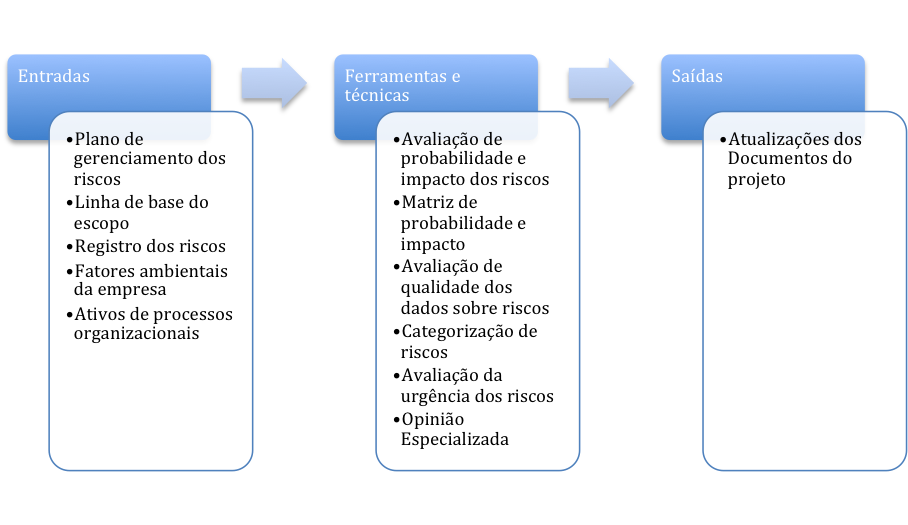
\includegraphics[scale=0.5]{Figuras/riscos_efts_analise_qual.png}
	\caption{Realizar a análise qualitativa dos riscos: entradas, ferramentas, técnicas e saídas}
	\label{fig:riscos:analise:qual:efts}
\end{figure}

\section{Entradas}

\begin{description}
	\item[Plano de gerenciamento dos riscos:] contém diversos elementos chave para análise dos riscos.
	
	\item[Linha de base do escopo:] auxilia na análise da complexidade do projeto.
	
	\item[Registro dos riscos:] contém informações para avaliar e priorizar os riscos.
	
	\item[Fatores ambientais da empresa:] estudos de especialista sobre riscos de projetos similares, bancos de dados de riscos, etc.
	
	\item[Ativos de processos organizacionais:] informações de projetos finalizados similares.

\end{description}

\section{Ferramentas e técnicas}

\begin{description}
		\item[Avaliação de probabilidade e impacto dos riscos:] investiga a probabilidade de cada risco específico ocorrer.
		
		\item[Matriz de probabilidade e impacto:] avaliação da importância e prioridade de atenção de cada risco é tipicamente conduzida usando uma tabela ou matriz de probabilidade e impacto.
		
		\item[Avaliação de qualidade dos dados sobre riscos:] avaliação do grau de utilidade dos dados sobre riscos.
		
		\item[Categorização de riscos:] os riscos podem ser categorizados pela fonte, área do projeto afetada ou outras categorias úteis.
		
		\item[Avaliação da urgência dos riscos:] riscos com respostas de curto prazo podem ser considerados mais urgentes.
		
		\item[Opinião Especializada:] auxiliam na avaliação da probabilidade  e impacto de cada risco.
		
\end{description}

\section{Saídas}

\begin{description}
	
	\item[Atualizações dos Documentos do projeto:] registro de riscos, registro de premissas, etc.
	
\end{description}

\secao{Realizar a análise quantitativa dos riscos}

Processo de efetuar a análise numérica do efeito dos riscos identificados nos objetivos gerais do projeto.

O processo de realizar a análise quantitativa dos riscos está representado na Figura \ref{fig:riscos:analise:quant:efts} e será descrito a seguir.

\begin{figure}[!h]
	\centering
	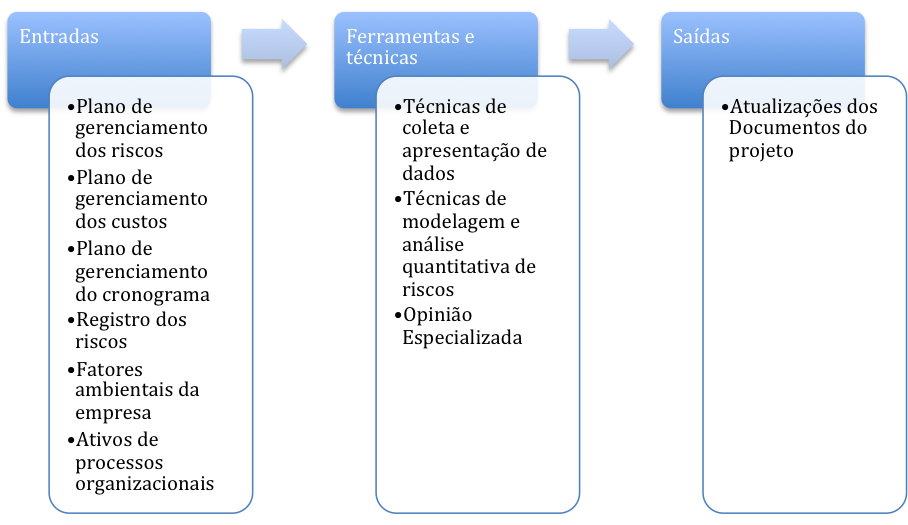
\includegraphics[scale=0.5]{Figuras/riscos_efts_analise_quant.png}
	\caption{Realizar a análise quantitativa dos riscos: entradas, ferramentas, técnicas e saídas}
	\label{fig:riscos:analise:quant:efts}
\end{figure}

\section{Entradas}

\begin{description}
	
	\item[Plano de gerenciamento dos riscos:] contém os guias, métodos e ferramentas utilizadas na análise quantitativa.
	
	\item[Plano de gerenciamento dos custos:] contém os guias para estabelecer e gerenciar as reservas de risco.
	
	\item[Plano de gerenciamento do cronograma:] contém os guias para estabelecer e gerenciar as reservas de risco.
	
	\item[Registro dos riscos:] ponto de referência para realizar a análise.
	
	\item[Fatores ambientais da empresa:] estudos realizados por especialistas sobre riscos similares, bancos de dados de riscos, etc.
	
	\item[Ativos de processos organizacionais:] informações sobre projetos finalizados similares.
	
\end{description}

\section{Ferramentas e técnicas}

\begin{description}

	\item[Técnicas de coleta e apresentação de dados:] entrevistas, distribuição de probabilidades, etc.
	
	\item[Técnicas de modelagem e análise quantitativa de riscos:] análise de sensibilidade, análise de valor monetário esperado, modelagem e simulação, etc.
	
	\item[Opinião Especializada:] auxilia na identificação de pontenciais custos e impactos no cronograma, na avaliação de probabilidades, etc.
	
\end{description}

\section{Saídas}

\begin{description}
	
	\item[Atualizações dos Documentos do projeto:] análise probabilística do projeto, probabilidade de atingir os objetivos de custo e tempo, lista priorizada de riscos quantificados, tendências nos resultados de análise quantitativa dos riscos, etc.	
	
\end{description}


\secao{Planejar as respostas aos riscos}

Processo de desenvolver opções e ações para aumentar as oportunidades e reduzir as ameaças aos objetivos do projeto.

O processo de planejar as respostas aos riscos está representado na Figura \ref{fig:riscos:resp:efts} e será descrito a seguir.

\begin{figure}[!h]
	\centering
	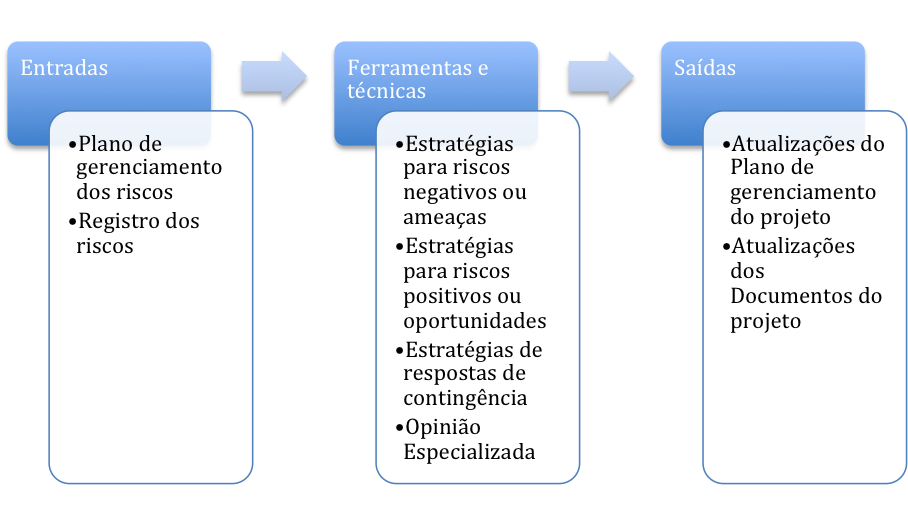
\includegraphics[scale=0.5]{Figuras/riscos_efts_resp.png}
	\caption{Planejar as respostas aos riscos: entradas, ferramentas, técnicas e saídas}
	\label{fig:riscos:resp:efts}
\end{figure}

\section{Entradas}

\begin{description}
	
	\item[Plano de gerenciamento dos riscos:] inclui papéis e responsabilidades, definições de análise de riscos, tempo para revisões, limites dos riscos, etc.
	
	\item[Registro dos riscos:] identifica os riscos, as causas raíz, lista de pontenciais respostas, etc.
	
\end{description}

\section{Ferramentas e técnicas}

\begin{description}
	
	\item[Estratégias para riscos negativos ou ameaças:] evitar, transferir, mitigar, aceitar.
	
	\item[Estratégias para riscos positivos ou oportunidades:] explorar, aumentar, compartilhar, aceitar.
	
	\item[Estratégias de respostas de contingência:] plano para respostas que serão executadas somente quando (e se) determinados eventos ocorrerem.
	
	\item[Opinião Especializada:] auxiliam com conhecimento sobre ações pertinentes às ações que devem ser tomadas para um determinado risco.
	
\end{description}

\section{Saídas}

\begin{description}
	
	\item[Atualizações do Plano de gerenciamento do projeto:] planos de gerenciamento do cronograma, custos, qualidade, aquisições e RH, além das linhas de base do escopo, cronograma e custo.
	
	\item[Atualizações dos Documentos do projeto:] diversos documentos auxiliares podem ser afetados pelas respostas aos riscos.	
	
\end{description}


\secao{Controlar os riscos}

Processo de monitorar e controlar os riscos durante o ciclo de vida do projeto.

O processo de controlar os riscos está representado na Figura \ref{fig:riscos:controlar:efts} e será descrito a seguir.

\begin{figure}[!h]
	\centering
	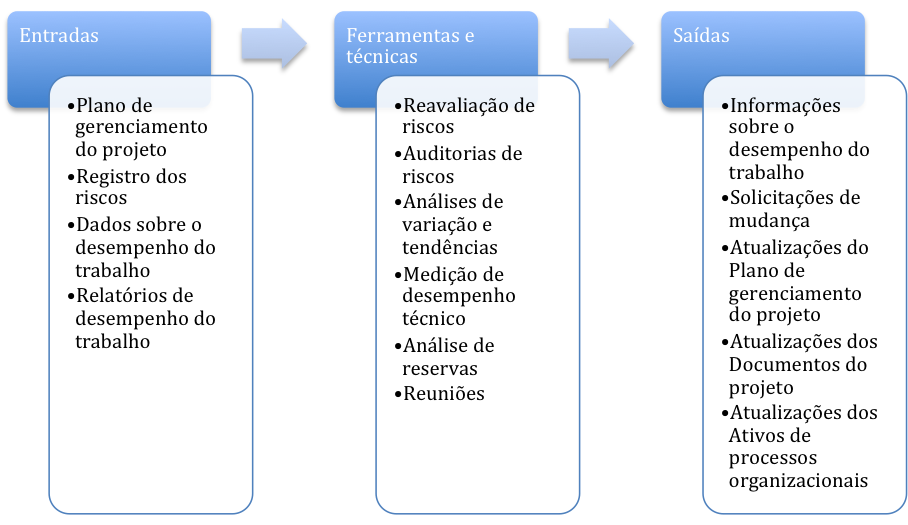
\includegraphics[scale=0.5]{Figuras/riscos_efts_controlar.png}
	\caption{controlar os riscos: entradas, ferramentas, técnicas e saídas}
	\label{fig:riscos:controlar:efts}
\end{figure}

\section{Entradas}

\begin{description}
	
	\item[Plano de gerenciamento do projeto:] contém guias para monitorar e controlar os riscos.
	
	\item[Registro dos riscos:] contém os riscos que devem ser monitorados e controlados.
	
	\item[Dados sobre o desempenho do trabalho:] status das entregas, progresso do cronograma, custos incorridos, etc.
	
	\item[Relatórios de desempenho do trabalho:] contém dados que podem impactar o controle de riscos relacionados com o desempenho.	
	
\end{description}

\section{Ferramentas e técnicas}

\begin{description}
	
	\item[Reavaliação de riscos:] o controle de riscos pode resultar na identificação de novos riscos.
	
	\item[Auditorias de riscos:] examina e documenta a efetividade das respostas aos riscos.
	
	\item[Análises de variação e tendências:] podem prever ponteciais desvios de custo e cronograma, indicadores de ponteciais riscos.
	
	\item[Medição de desempenho técnico:] podem prever o nível de sucesso para alcançar o escopo do projeto.
	
	\item[Análise de reservas:] compara a quantia da reserva de contingência remanescente com os riscos remanescentes para verificar se a reserva é suficiente.
	
	\item[Reuniões:] o gerenciamento de riscos deve constar da agenda de reuniões periódicas de desempenho.
	
\end{description}

\section{Saídas}

\begin{description}
	
	\item[Informações sobre o desempenho do trabalho:] oferece um mecanismo para comunicar e auxiliar o processo de tomada de decisão do projeto.
	
	\item[Solicitações de mudança:] ações corretivas e preventivas recomendadas.
	
	\item[Atualizações do Plano de gerenciamento do projeto:] planos de gerenciamento do cronograma, custos, qualidade, aquisições e RH, além das linhas de base do escopo, cronograma e custo
	
	\item[Atualizações dos Documentos do projeto:] saídas de avaliação de riscos, auditorias de riscos, revisões periódicas de riscos e saídas reais dos riscos e respostas.
	
	\item[Atualizações dos Ativos de processos organizacionais:] modelos do plano de gerenciamento de riscos, estrutura analítica de riscos, lições aprendidas, etc.
	
\end{description}